


\section{Problem Setup}
\label{sec:setup}

We formalize the task of localizing the decisive error in a failed agent
trajectory.

\textbf{Agent trajectory.}
Let $x$ denote a task description and
$\traj=(s_1,\ldots,s_T)$ the resulting trajectory of a multi-agent system.
Each step $s_t$ records the action or message produced at turn $t$ and is
associated with an agent $a_t\in\{1,\ldots,K\}$.
For evaluation, each failed trajectory is paired with a gold decisive-error
index $t^\star\in\{1,\ldots,T\}$, defined as the earliest step at which the
error responsible for the eventual task failure is introduced~\citep{whoandwhen}.
The corresponding responsible agent is $a_{t^\star}$.


Our framework extracts model-internal signals, including hidden
representations, using a frozen language model
$\proxy$.
When the language model underlying the agents exposes its internal states,
$\proxy$ may coincide with that model.
Otherwise, $\proxy$ can be a separate open-weight model, enabling the
analysis of trajectories generated by proprietary agents whose internal
states are inaccessible.
In either case, $\proxy$ is used without fine-tuning on failure-attribution
data.

\textbf{Failure attribution.}
Given a task description $x$ and a failed trajectory $\traj$, the goal is to
estimate its decisive-error index $t^\star$.
We operationalize this prediction by assigning each step a scalar attribution
score $\Stilde(s_t)\in\mathbb{R}$, where a larger value indicates stronger
evidence that $s_t$ introduced the failure.
The predicted decisive-error step and responsible agent are
$
    \hat{t}
    =
    \arg\max_{t\in\{1,\ldots,T\}}
    \Stilde(s_t),
    \hat{a}
    =
    a_{\hat{t}}.
$
Sorting these scores additionally produces a ranked list of candidate steps
for failure triage.
We evaluate both top-1 localization and top-$k$ performance in
Section~\ref{sec:exp:main} and Appendix~\ref{app:ranked}, respectively.

\textbf{Step-unlabeled failure trajectories.}
In addition to the test trajectory, we assume access to a disjoint reference
collection of failed trajectories
$
    \mathcal{D}_{\mathrm{fail}}
    =
    \left\{
        \bigl(x^{(n)},\traj^{(n)}\bigr)
    \right\}_{n=1}^{N},
    \traj^{(n)}
    =
    \bigl(s^{(n)}_1,\ldots,s^{(n)}_{T_n}\bigr).
$
The task-level outcome of every reference trajectory is known to be a
failure, but no step-level annotation identifies where the failure was
introduced or which agent was responsible.
We model the  marginal distribution of reference steps as an unlabeled
contamination mixture~\citep{huber1964robust}:
\begin{equation}
\small
    P_{\mathrm{unlabeled}}
    =
    (1-\phi)P_{\mathrm{ord}}
    +
    \phi P_{\mathrm{err}},
    \label{eq:step-contamination}
\end{equation}
where $P_{\mathrm{ord}}$ denotes the distribution of ordinary steps,
$P_{\mathrm{err}}$ denotes that of failure-related steps, and
$\phi\in(0,1)$ is the unknown contamination proportion.
Failure-related steps include the decisive error and any downstream steps
affected by it. Formally, each reference trajectory has an unobserved nonempty set
$\mathcal{E}^{(n)}\subseteq\{1,\ldots,T_n\}$ of failure-related steps, whose
earliest member is the decisive-error step:
$
    t^{\star(n)}
    =
    \min\mathcal{E}^{(n)}.
$
At the marginal level,
$s_t^{(n)}\sim P_{\mathrm{err}}$ when
$t\in\mathcal{E}^{(n)}$ and
$s_t^{(n)}\sim P_{\mathrm{ord}}$ otherwise.
This setting is \textit{practical} because failed trajectories can often be collected
automatically using task-level evaluators, whereas localizing the decisive
error and assigning responsibility require costly expert annotation.

Our method uses $\mathcal{D}_{\mathrm{fail}}$ only to construct the reference
representation space, without observing $\mathcal{E}^{(n)}$ or any
responsible-agent annotations.
Gold step-level labels are reserved for evaluation and, where applicable,
hyperparameter selection on a disjoint validation split.





\begin{figure}[t]
\centering
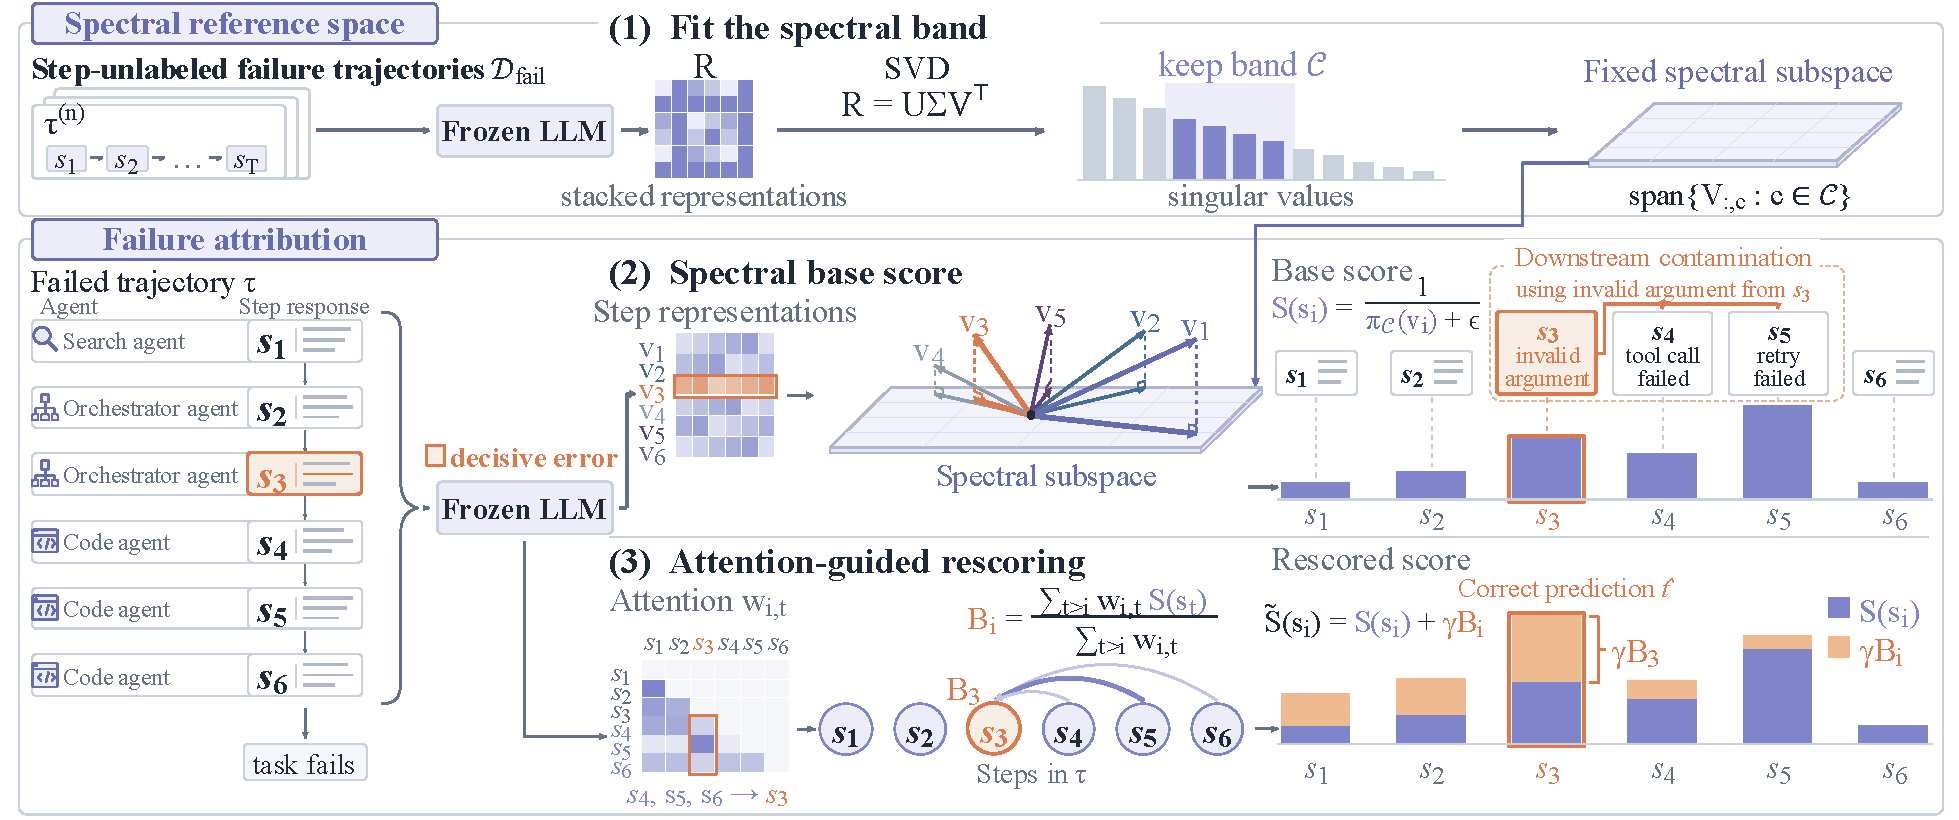
\includegraphics[width=\textwidth]{assets/soap_framework_v48.pdf}
  \vspace{-0.6cm}
  \caption{\small 
  \textbf{Overview of \soap for agentic failure attribution.} \soap constructs a spectral reference space from step-unlabeled failure trajectories and assigns each step a base error score. To address downstream contamination, \soap derives soft dependencies from attention patterns and propagates downstream error evidence toward likely upstream sources to localize the decisive error.
  % \emph{During fitting}, a frozen proxy model $\proxy$ encodes every step of the
  % unlabeled reference failures $\mathcal{D}_{\mathrm{fail}}$, and the SVD of the
  % stacked representations yields a spectral band $\mathcal{C}$ capturing the
  % common mode of ordinary steps, onto which decisive errors project weakly.
  % \emph{During localization}, the same proxy encodes the failed trajectory:
  % each step receives the spectral base score      
  % $\Sbase(s_t)=1/(\pi_{\mathcal{C}}(v_t)+\epsilon)$, and attention-derived 
  % dependency weights $w_{i,t}$ propagate downstream error evidence back to the
  % predecessors it builds on, moving the argmax of the rescored $\Stilde$ from a
  % late symptom onto the decisive error $t^\star$; the responsible agent follows
  % as $\hat{a}=a_{\hat{t}}$. \soap{} involves no step labels, fine-tuning, or
  % LLM prompting. 
  % \note{New layout for the main figure. Under refinement: too much text, need more compact, avoid overlapping components.}
  % \textcolor{red}{the fonts are not proper, please avoid purely relying AI for this. characters are stitched together.} 
  }
\label{fig:overview}
\vspace{-0.5cm}
\end{figure}

% Eqn.~\ref{eq:step-contamination} characterizes the marginal composition of the pooled steps; it does not assume that steps within a trajectory are temporally independent.


% \textbf{Per-step scoring formulation.}





% \section{Problem Setup}
% \label{sec:setup}

% Let $\traj = (s_1, \ldots, s_T)$ be a trajectory of a turn-based multi-agent system, with each step $s_t$ attributed to an agent $a_t \in \{1, \ldots, K\}$. A failed trajectory is annotated with a \emph{decisive-error step} $t^\star \in \{1, \ldots, T\}$---the earliest step at which an irrecoverable mistake was introduced---and the responsible agent $a_{t^\star}$. Given $\traj$ and the task description, the failure-attribution task~\citep{whoandwhen} is to predict $\hat{t}$ as an estimator of $t^\star$, with the corresponding agent prediction $\hat{a} = a_{\hat{t}}$.

% We assume access to a proxy language model $\proxy$, distinct from the model that generated $\traj$, exposing intermediate hidden states and post-softmax attention probabilities. $\proxy$ is used without adaptation or supervision on failure-attribution data. This setting reflects practice: trajectories are often produced by proprietary models whose internals are inaccessible, whereas open-weight proxies are freely inspectable.

% \paragraph{Per-step scoring view.} Rather than predicting $\hat t$ directly, we produce a scalar score $\Stilde(s_t)\in\mathbb{R}$ for every step and rank within the trajectory, so that
% \begin{equation}
%   \hat{t} \;=\; \arg\max_{t \in \{1,\ldots,T\}}\; \Stilde(s_t),
%   \label{eq:prediction}
% \end{equation}
% and the top-$k$ scored steps form a ranked candidate set for triage. We report both the top-1 prediction in \eqref{eq:prediction} and ranked-set metrics (\S\ref{sec:experiments}).
